\part{Détection d'anomalies}
\label{prt:detection}

\chapter{La détection d'anomalies par Isolation} 

\section{Méthode d'isolation des anomalies}

Dans un ensemble de données, les anomalies peu nombreuses avec des caractéristiques très différentes.

La détection d'anomalies, consiste à isoler ces données rares et fortement différentes d'une base de données. C'est un concept utilisé dans différents domaines comme la sécurité informatique (détection d'intrusion, ),.

Il existe une multitude de méthodes de détection d'anomalies, toutes basées en générale sur les calculs de distance ou de noyaux. Ces méthodes supposent que des données "normales" auront tendance à être fortement groupées, rapprochées et les données qui sont éloignées d'un ou de plusieurs groupes de données sont considérées comme des anomalies.

Sachant que dans un ensemble de données, les anomalies sont plus ou moins très rares et différentes, la méthode procède par isolation pour détecter ses anomalies. L'isolation consiste à construire un arbre de décision à partir des données jusqu'à ce que chaque individu soit dans une et une seule feuille.

Une fois que les données sont isolées dans l'arbre de décision ou d'isolation, la probabilité qu'une donnée soit une anomalie est quantifiée par sa profondeur dans l'arbre. Une données qui a été isolée très vite lors de la construction de l'arbre de décision a plus de probabilité d'être une anomalie.

Pour effectuer la détection d'anomalies par isolation, on choisi au hasard un échantillon dans une base de données, ensuite on choisi des variables au hasard parmi les variables de l'échantillon et on déroule un arbre de décision.

%On répète cette méthode n fois, on crée donc $n$ arbres d'isolation %et d'échantillons différents tous tirés des données initiales. %L'ensemble de ces arbres d'isolations est appelé forêt d'isolation.

\section{Phase d'apprentissage}

La phase d'apprentissage consiste à construire un ensemble d'arbre soit des \emph{iTree}, sur les données pour créer une forêt d'isolation, les \emph{iForest}.

Le principe est relativement simple, et s'effectue essentiellement en deux phases dont la première sera la construction de l'arbre de décision, puis par bootstrapping la construction de la forêt de décision.

\subsection*{Construction de l'arbre de décision}

La construction de l'arbre d'isolation se fait par échantillonnage sur les deux dimensions, variables et individus.
Considérons la base de données  suivante :
Elle est formée de $m$ individus $I$ et de $n$ variables $V$.

\begin{table}[H]
\centering
\caption{Base de données}
\label{bdd}
\begin{tabular}{|l|l|l|l|l|}
\hline
 & $V_1$ & $V_2$ & $\cdots$ & $V_n$ \\ \hline
$I_1$ &  &  &  &  \\ \hline
$I_2$ &  &  &  &  \\ \hline
$\vdots$ &  &  &  &  \\ \hline
$I_m$ &  &  &  &  \\ \hline
\end{tabular}
\end{table}

Premièrement, un échantillonnage est effectué de façon aléatoire, sur les individus et sur les variables qui les caractérisent.

\begin{table}[H]
\centering
\caption{Échantillon}
\label{ech}
\begin{tabular}{|l|l|l|l|}
\hline
 & $V_1$ &  $\cdots$ & $V_n$ \\ \hline
$I_1$ &  &  &  \\ \hline
$\vdots$ &  &  &  \\ \hline
$I_m$ &  &  &  \\ \hline
\end{tabular}
\end{table}

A partir de l'échantillon choisi de façon aléatoire, un arbre d'isolation (décision) est construit, de telle sorte que chaque individu se trouve seul sur une feuille au bout de l'arbre. c'est la condition d'arrêt de la construction d'un arbre, mais toute fois elle peut être manipulée de telle sorte à pouvoir arrêter la construction d'un arbre trop profond.

Dans la phase d'apprentissage, trois paramètres sont donc nécessaires pour le déroulement de l'algorithme : 

\begin{itemize}
    \item $X$ : les données
    \item $\psi$ : la taille de l'échantillon
\end{itemize}

La taille de l'échantillon $\psi$ permet de contrôler la taille des données d'apprentissage. C'est un paramètre qui joue donc notamment sur la profondeur de l'arbre d'isolation et donc sur la performance de la méthode d'isolation. Par ailleurs, à partir d'une certaine taille, les performances de détections tendent à devenir constante, généralement $\psi=256$ est suffisant pour effectuer une détection d'anomalie dans une base de données.

\subsection*{Construction de la forêt d'arbre de décision}
Une forêt d'arbre de décision est composée de plusieurs arbres de décision. Sa construction s'effectue en ré-échantillonnant plusieurs fois avec la construction d'un arbre par échantillon. Ainsi, un autre paramètre vient s'ajouter aux deux autres, $t$ qui désigne le nombre d'arbre qui compose la forêt. En générale, le chemin d'isolation d'un individu dans un arbre converge avant la construction de $t=100$ arbres.
\\
\\
La complexité dans le pire des cas ce la phase d'apprentissage est de $O(t\psi^2)$ et temps, et de $O(t\psi)$ en espace.

\section{Phase d'évaluation}
La phase d'évaluation consiste à calculer le taille moyenne du chemin d'isolation d'un individu sur l'ensemble de la forêt.
La taille $h(x)$ du chemin d'un individu $I$, correspond au nombre de noeuds $e$, entre la base de l'arbre d'isolation et le noeud d'extrémité (bout de l'arbre) où cet individu a été isolé. 
Lorsque la taille du chemin d'isolation d'un individu dépasse une certaine limite $hlim$ prédéterminée, la taille du chemin est estimée par $hlim+c(Size)$, avec $c(Size)$ une valeur d'ajustement \footnote{\cite{Liu2012}}.
\\
\\
La complexité dans le pire des cas ce la phase d'évaluation est de $O(nt\psi)$ et temps, avec $n$ le nombre de test.

\section{Les anomalies et leurs scores}

Un score, pour déterminer le degré d'anormalité d'un individu est essentiel à toute méthode de détection d'anomalie.
Le score $s$ d'un individu I se calcul comme :
\begin{equation}
    s(I,\psi)=2^\frac{E(h(x))}{c(\psi)}
\end{equation}

\begin{itemize}
    \item $E(h(x))$ est la moyenne des tailles du chemin d'isolation d'un individu I dans une forêt d'isolation.
    \item $c(\psi)$ désigne la moyenne des $h(x)$ dans un échantillon
\end{itemize}

Dans certaines conditions la valeur du score est directement déduite :
\begin{itemize}
    \item $E(h(x)) \rightarrow 0,  s \rightarrow 1;$
    \item $E(h(x)) \rightarrow \psi-1,  s \rightarrow 0; $
    \item $E(h(x)) \rightarrow c(\psi),  s \rightarrow 0.5;$
\end{itemize}

En posant :

\begin{equation}
    s(I,\psi)=0,5 - 2^\frac{E(h(x))}{c(\psi)}
\end{equation}

plus le score est faible plus la probabilité d'être une anomalie est grande.

\chapter{Application}

Ce chapitre se consacre à une application pratique de la détection d'anomalies dans un contexte de finance de marché et de gestion du risque. 

Maintenant que nous disposons d'un algorithme peu coûteux en temps et en mémoire, on peut poser des hypothèses de détection d'anomalies que nous allons appliquer à des données financières de marchée volumineuse, pour en détecter ce qui s'éloignent de la norme. Dans un certain contexte on ne parlera pas d'anomalies bien que nous appliquons une méthode de détection d'anomalie, mais plutôt de particularité.

\section{Le Standard \& Poor's 500}

Le Standard \& Poor's 500 ou S\&P 500 est un indice bousier basé sur un peu plus de 500 grandes sociétés cotées sur les bourses des États-Unis.
\\
\\
Considérons l'historique des prix de clôture du marché de l'ensemble des actifs de l'indice entre le 11 Août 2015 et le  11 Août 2017. L'objectif de cette application, sera de détecter parmi les 500 actifs, les quelques uns qui ont des comportements très particuliers sur le marché.
\\
\\
Cependant, il est nécessaire de noter que les interprétations sur les actifs anormaux dépendent fortement des variable qui caractérisent les actifs. Une donnée peut être identifiée pour être anormale, mais l'essentiel sera de savoir dans quelle contexte elle est anormale.
\\
\\
En fonction du type d'anomalie que l'on veut identifier, il faut veiller à travailler sur les bonnes variables, au risque de considérer des anomalies et résoudre les mauvais problèmes.
\\
\\
Notre objectif sera de détecter des actifs qui présentent des distributions de rendement anormaux sachant que par hypothèse les rendements historiques d'un actif suivent une loi normale centrée en zéro, c'est à dire que son espérance est nulle, avec une volatilité proportionnelle au temps. L'objectif de cette application est de savoir si il existe des actifs de l'indice S\&P 500 qui présentent une loi normale de caractéristique extrême par rapport aux autres, synonyme de plus ou moins de risque.

\section{Isolation sur le Standard \& Poor's 500}

Soit les 500 actifs qui composent l'indice S\&P 500. 
Considérons l'historique des prix de clôture des actifs entre le 11 Août 2015 et le  11 Août 2017.
Cette application porte sur une étude des distributions des rendements de ces actifs, sachant que le rendement d'un actif suit une loi normale. 

\subsection{Les rendements}

Le graphique suivant montre l'évolution des rendements moyens entre le 11 Août 2015 et le 11 Août 2017. Le rendement moyen est le rendement journalier sur lequel on applique une moyenne mobile avec une fenêtre de quarante jours.

\begin{figure}[H]
\centering
\caption{Moyenne mobile des rendements}
   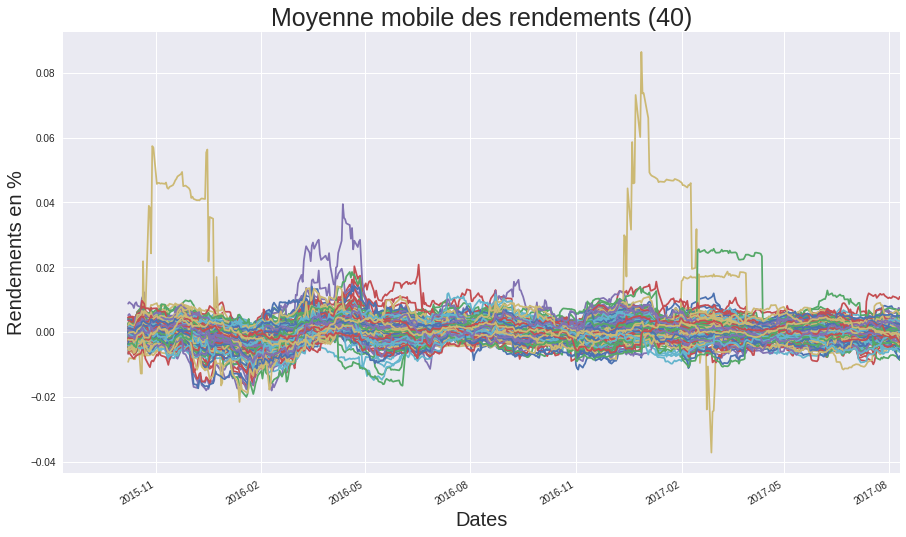
\includegraphics[scale=0.5]{img/rendements.png}
\end{figure}

Ce graphique est touffu et pratiquement illisible, on a superposé 500 courbes et on en distingue clairement aucune. Cependant, en regardant hors des surcharges, on peu remarquer quelques courbes qui se distinguent fortement avec des piques bien au dessus et ou au dessous de la moyenne des autres. Ce sont ces genres d'actifs que l'on veut détecter, les actifs avec un profil historique de rendement moyen totalement différent voir exceptionnel des autres. Une fois détecté, un ensemble d'étude peuvent être menées pour interpréter ces résultats.

\subsection{Les volatilités}

Le graphique suivant montre l'évolution des volatilités des rendements moyens entre le 11 Août 2015 et le 11 Août 2017. La volatilité moyenne mobile sur une fenêtre de quarante jour.

\begin{figure}[H]
\centering
\caption{Volatilité des actifs}
   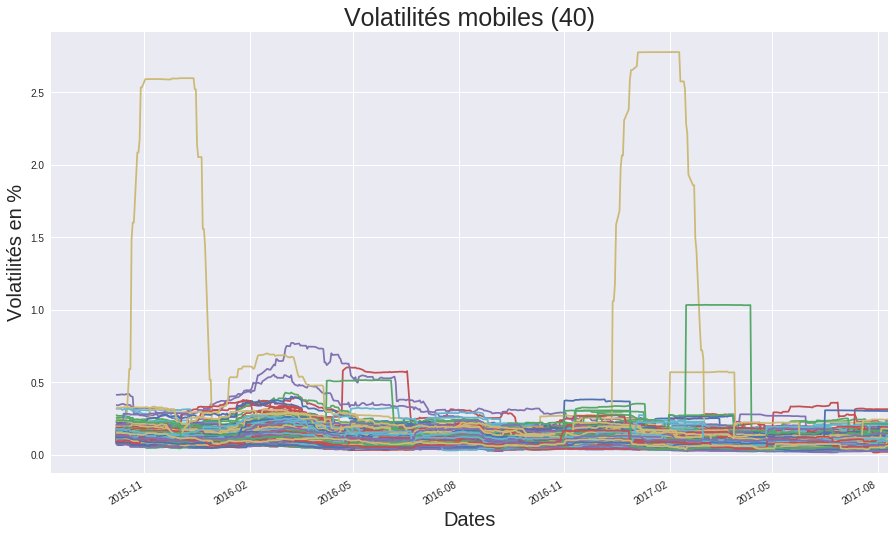
\includegraphics[scale=0.5]{img/volatilites.png}
\end{figure}

On observe une masse bien dense de courbe qui se superposent puis quelques unes qui se démarquent clairement par endroit.
Sachant que la volatilité d'un actif détermine le niveau de risque de ce actif, il n'est pas exagéré de vouloir porter un œil sur ce actif afin d'en évaluer efficacement le risque.

\subsection{Densité de probabilité des rendements}

Les rendements d'un actif suivent une loi normale centrée en 0 avec une certaine volatilité.  Les paramètres donc de volatilité et de rendements caractérisent la densité de la loi que suivra les rendements. C'est à dire qu'en étudiant la fonction de densité des rendements des actifs on porte aussi un œil sur ses deux premiers paramètres

La fonction de densité d'un actif dans cette application à été approximé de manière non paramétrique par la méthode d'estimation par noyaux\footnote{ Méthode de Parzen-Rosenblatt (wikipedia)}. Cette méthode est implémentée dans trois bibliothèque python et sont accessible de façon simple.

En utilisant cette méthode pour obtenir la courbe des distributions et en les superposant il est difficile de voir les différences entre les différentes distributions, elles ont l'air homogènes et de loi normale.

\begin{figure}[H]
\centering
\caption{Distribution des rendements}
   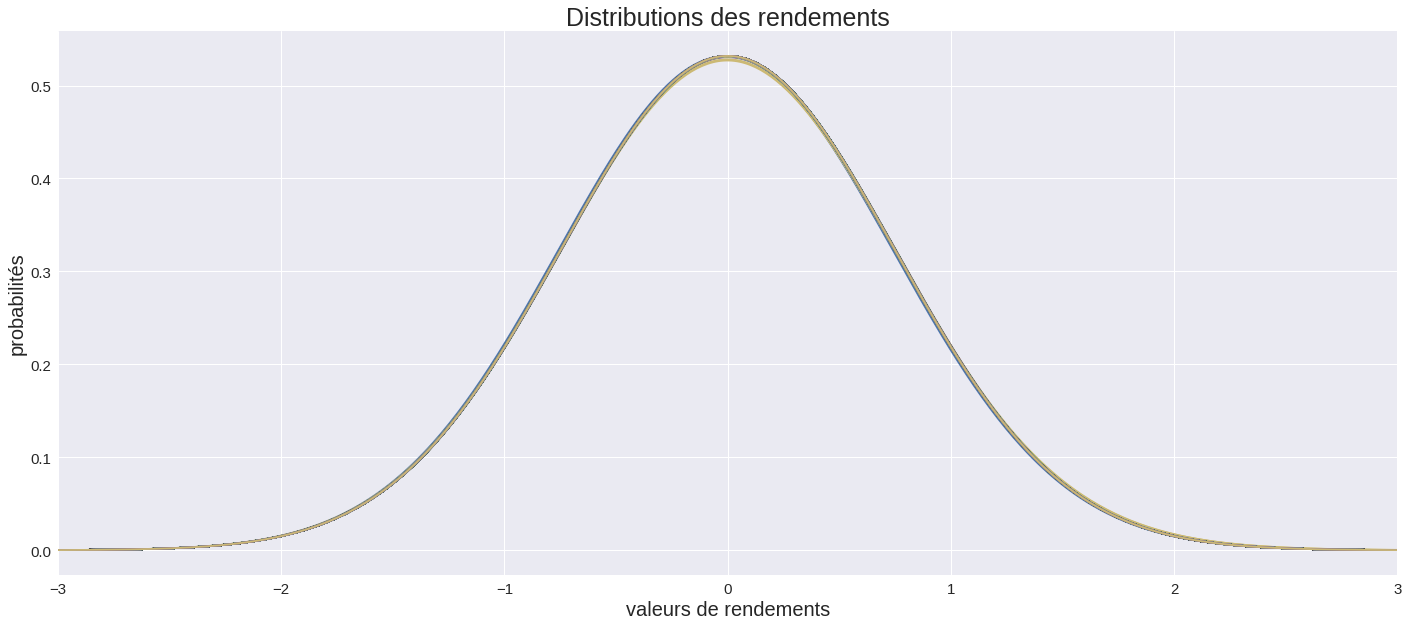
\includegraphics[scale=0.35]{img/distrib.png}
\end{figure}

\subsection{Densité par la méthode des histogrammes}

En regardant de plus près, en visualisant de façon empirique les différentes distributions, en utilisant un graphique d’histogramme lissé on aperçoit qu'en réalité les loi de probabilités des rendements sont différentes. Les différences se situent notamment soit à la base, au sommet et à la forme. Certaines distributions sont plus effilées que d'autres. 

La figure ce dessous illustre les différences de distribution de rendements entre 4 quatre  actifs qui composent le S\&P 500 choisies aléatoirement.

Ces actifs sont listés dans le tableau \ref{actif}.

\begin{table}[H]
\centering
\caption{Actifs du S\&P 500}
\label{actif}
\begin{tabular}{|l|}
\hline
A : Agilent Technologies Inc \\
AKAM : Akamai Technologies Inc \\
ADSK : Autodesk Inc \\
AAP : Advance Auto Parts \\ \hline
\end{tabular}
\end{table}

\begin{figure}[H]
\centering
\caption{Distribution des rendements}
   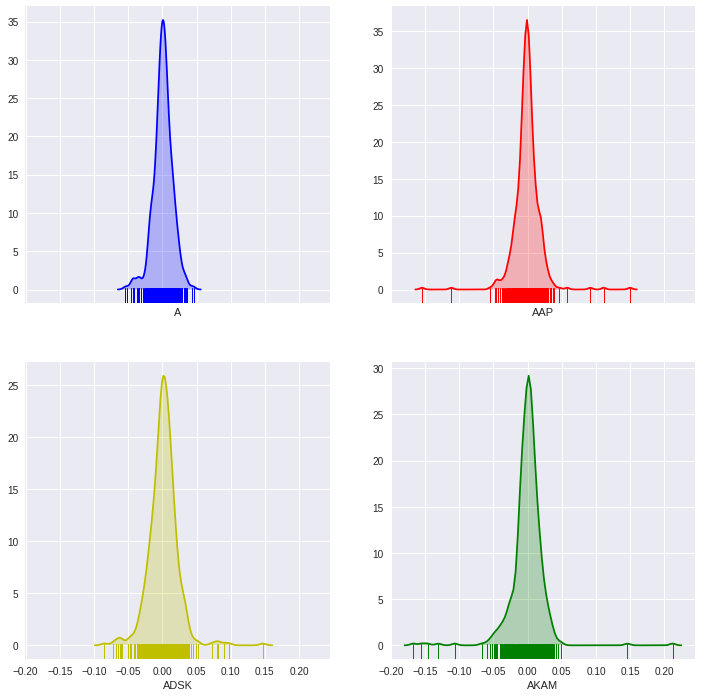
\includegraphics[scale=0.7]{img/distrib2.png}
\end{figure}

On peut noter que la loi des rendements n'est pas exactement normale, c'est une hypothèse, avec pour principale conséquence un biais dans la quantification de risque, notamment dans le calcul d'indicateur la Value at Risk (VaR).

Ces différentes courbes, apporte une précision sur la loi de probabilité des rendements de chaque actif avec les différences qui peuvent exister entre elles. Des différences qui peuvent principalement être interprétées comme une comparaison du niveau de risque. Certains actifs seront plus risqués que d'autres, et ceux qui présentent soit des niveaux de risque extrêmes (faibles ou élevé) peuvent être intéressant à détecter. C'est ainsi qu'intervient la détection d'anomalie, par une méthode qui va isoler ces actifs "particuliers", c'est à dire ceux avec un profil de rendement différent.

\section{Isolation des actifs}

La méthode de détection d'anomalie par isolation est implémentée  dans une librairie de machine learning python qui est Scikitlearn sous le nom de \emph{sklearn.ensemble.IsolationForest} \footnote{Documentation : http://scikit-learn.org/stable/modules/generated/sklearn.ensemble.IsolationForest.html\#id1}. 

Deux approches seront utilisées pour isoler les actifs qui présentent des "anomalies" de rendement. Une approche standard, directement appliquée sur la distribution des rendements puis une autre approche basée sur la forme de courbe de la distribution des rendements.

\subsection{Isolation des distributions}

En appliquant la méthode de détection d'anomalies par isolation,on obtient les actifs qu'elle aura isolé et qui donc présentent des différences signifiantes. Pour isoler ces actifs elle se base sur le score de chaque actif, ceux avec les scores les plus faibles ont une forte probabilité d'être des anomalies.

Ainsi l'ensemble des scores pour l'ensemble des actifs sont : 


\begin{figure}[H]
\centering
\caption{Scores de l'ensemble des actifs}
   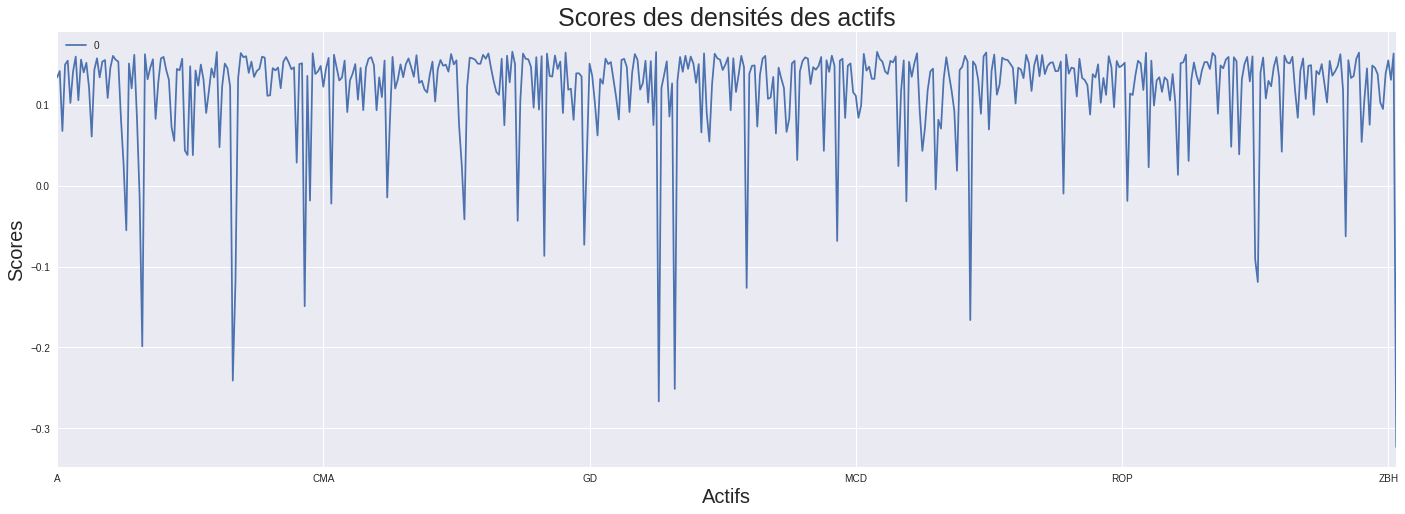
\includegraphics[scale=0.35]{img/scores_densite_all.png}
\end{figure}

Les scores des anomalies probables identifiées par la méthode se présente graphiquement comme ceci : 

\begin{figure}[H]
\centering
\caption{Scores des anomalies isolées}
   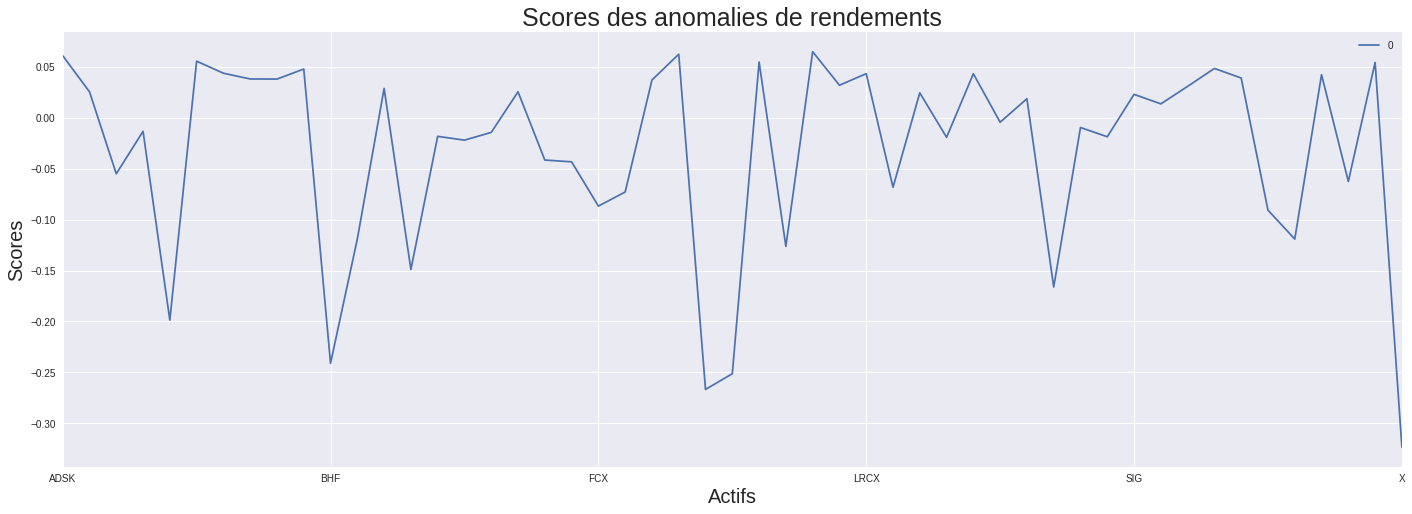
\includegraphics[scale=0.35]{img/scores_densite.png}
 \label{scoredensite}
\end{figure}

En conclusion la liste des anomalies identifiées avec leurs scores dans la figure \ref{scoredensite} est la suivante : 

['ADSK', 'ALB', 'ALGN', 'AMAT', 'AMD', 'APC', 'ARNC', 'ATVI', 'AVGO',
       'BBY', 'BHF', 'BHGE', 'CF', 'CHK', 'CHTR', 'CMG', 'CTXS', 'DVN', 'DXC',
       'EVHC', 'FCX', 'FTI', 'FTV', 'GILD', 'HLT', 'HPQ', 'INCY', 'JEC', 'KMI',
       'LB', 'LRCX', 'M', 'MOS', 'MRO', 'MU', 'NEM', 'NRG', 'NVDA', 'PRGO',
       'RRC', 'SIG', 'SRCL', 'STX', 'TRIP', 'TSCO', 'UA', 'UAA', 'URI', 'WMB',
       'WYNN', 'X']\footnote{ Les significations de ces abbréviations peuvent être trouvés sur http://www.zonebourse.com/S-P-500-4985/composition/}

\subsection{Identification des différences}

On retient donc que ces actifs listés ci dessus présenteront des distributions peu communes de l'ensemble des 500 actifs du S\&P 500 considérés au départ.
Maintenant clarifions un peu le tout par une comparaison entre distribution "normale" et "anormale".

Soit les actifs anormaux qui ont été isolés 'ALGN' et 'ADSK'. 
\\
Soit les actifs normaux 'A' et 'ABBV'.

Une comparaison des distributions de ces quatre actifs donne le graphique suivant : 

\begin{figure}[H]
\centering
\caption{Comparaison entre actifs "anormales" et "normals"}
   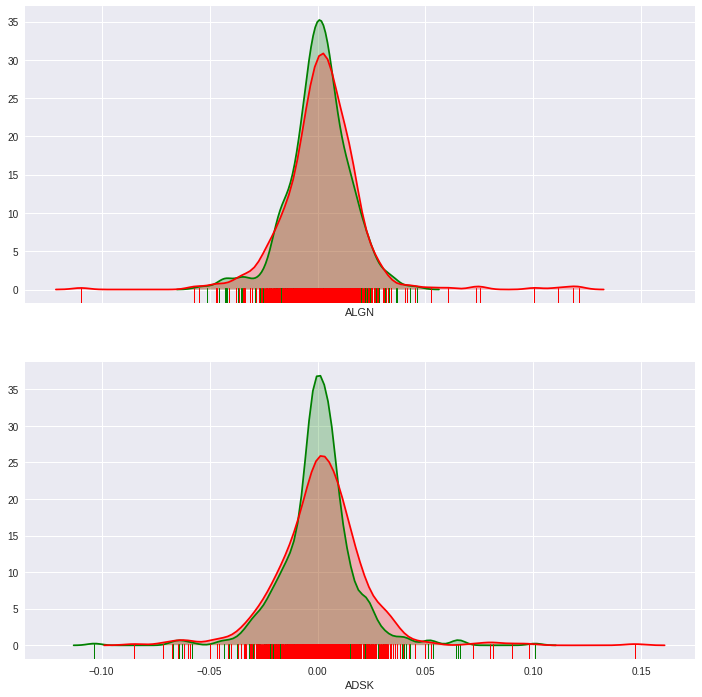
\includegraphics[scale=0.7]{img/anomalie_vs_normal.png}
 \label{anorm}
\end{figure}

Les courbes en vert présentent les distributions normales, et ceux en rouge les distributions isolées. La différence peut être résumé  comme suit :
\begin{itemize}
\item Les distributions normales (en vert dans la figure \ref{anorm}) ont des courbes avec une base fine, mais élancées en zéro
\item  Les distributions anormales (en rouge dans la figure \ref{anorm}) ont des courbes plus tassées en zéro avec une base plus épaisse.
\end{itemize}

A partir de ces différences identifiées, entre distribution de rendement normales et anormales on peu porter un ensemble d'interprétation sur ces allures et en identifier les conséquences.
La détection d'anomalie a été significative, elle a permit d'indexer directement des distributions de rendement particulières dans un ensemble, sans avoir à les comparer deux à deux.

\section{Isolation des actifs avec Nielson-Siegel-Svensson}

L'isolation par Nielson siegel svensson Consiste à recommencer le procédé de la section précédente savec différentes donnée. En effet, les distribution de probabilités sont passées à NSS, qui retourne les 6 coefficients pour chaque distribution qui résument la forme de sa courbe\footnote{L'application de la méthode de NSS sur l'historique des rendements pour les 500 actifs a duré 2 heures, pour un processeurs i7 quand core 2.6GHz }. On passe d'un historique de rendement sur deux ans, à essentiellement 6 variables sur lesquelles on applique la méthode de détection par isolation.

Il est important de préciser que les lois des rendements ont été estimées de façon non paramétrique en utilisant la méthode du noyau (méthode de Parzen-Rosenblatt).

On obtient les résultats suivants :

Score de l'ensemble des courbes de distribution.

\begin{figure}[H]
\centering
\caption{Scores de l'ensemble des distribution (NSS)}
   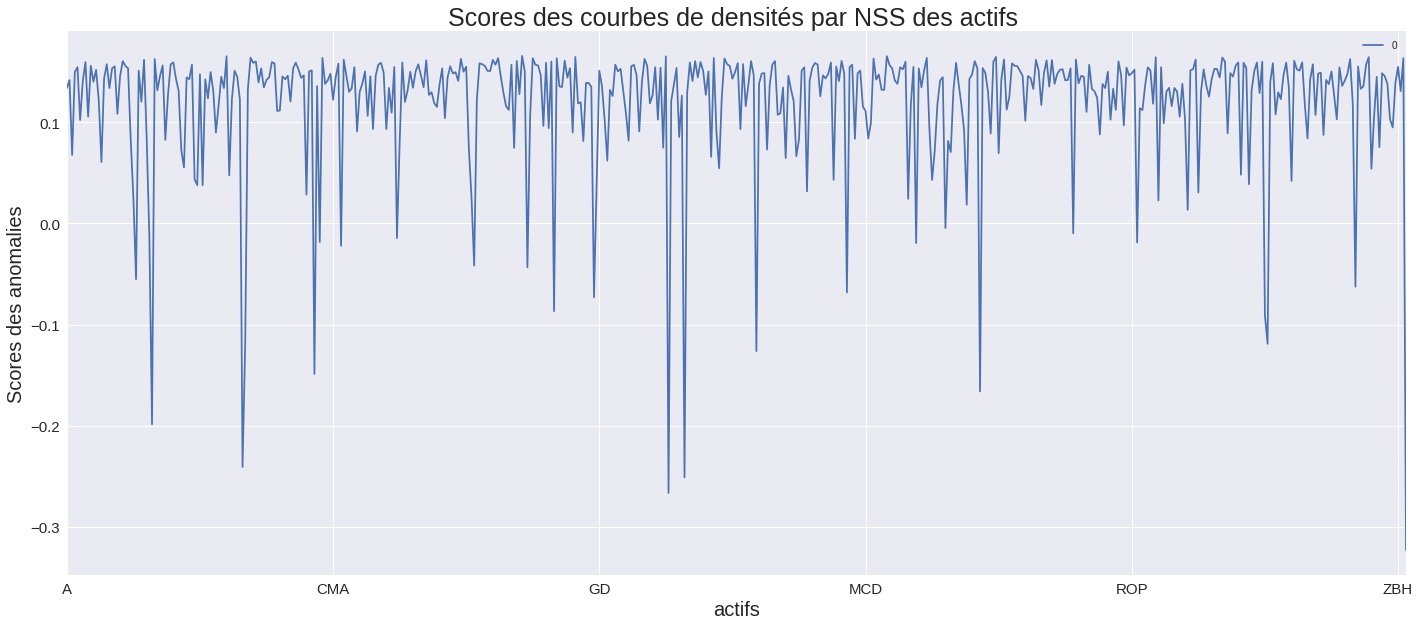
\includegraphics[scale=0.35]{img/scores_densite_nss_all.png}
 \label{anormm2}
\end{figure}

Score des anomalies isolées par la méthode de détection :

\begin{figure}[H]
\centering
\caption{Comparaison entre actifs "anormaux" et "normaux" (NSS)}
   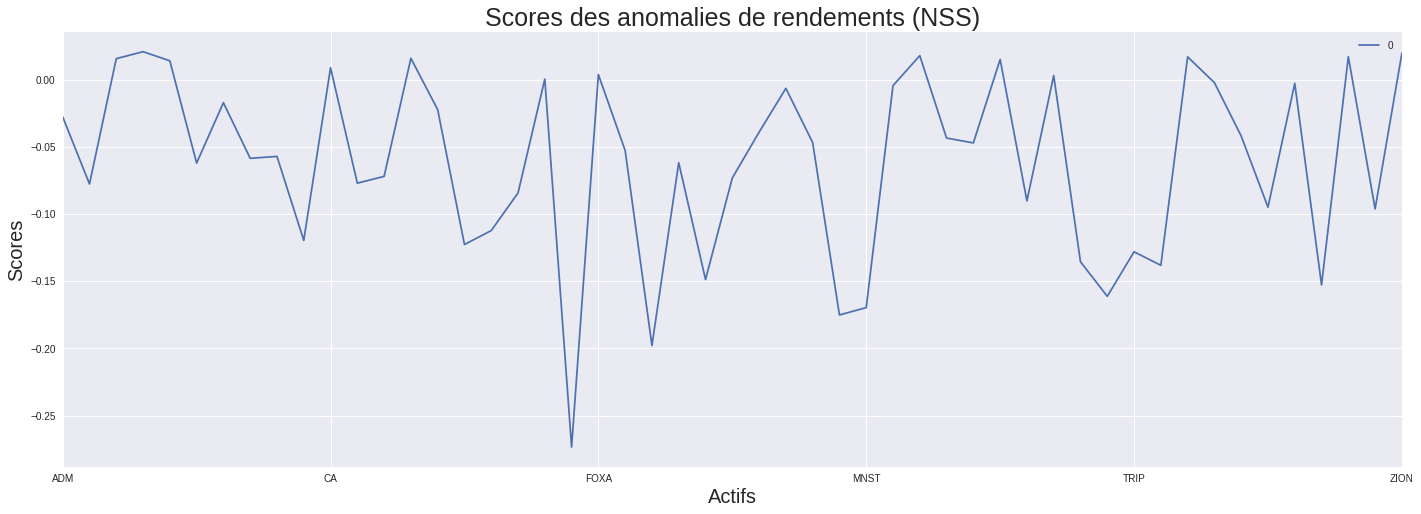
\includegraphics[scale=0.35]{img/scores_densite_NSS.png}
 \label{anormm1}
\end{figure}

Liste des actifs isolés :

['ADM', 'AFL', 'ALL', 'APC', 'APD', 'AVGO', 'BHF', 'BHGE', 'BK', 'BMY',
       'CA', 'CB', 'CHK', 'CME', 'CSX', 'DRE', 'DVN', 'ETN', 'EXC', 'FISV',
       'FOXA', 'GILD', 'GRMN', 'HLT', 'HPQ', 'JNJ', 'KSU', 'LB', 'LEG', 'M',
       'MDT', 'MNST', 'MRO', 'NOC', 'OKE', 'ORLY', 'PAYX', 'PFE', 'PSX', 'RRC',
       'SNA', 'TMO', 'TRIP', 'TROW', 'VTR', 'WMB', 'WMT', 'WYNN', 'XLNX',
       'ZBH', 'ZION']

Comparaison entre distributions normales en vert (A,ABBV) et anormales en rouge (ADM, ZION) sur la figure suivante:

\begin{figure}[H]
\centering
\caption{Comparaison entre actifs "anormales" et "normals" (NSS)}
   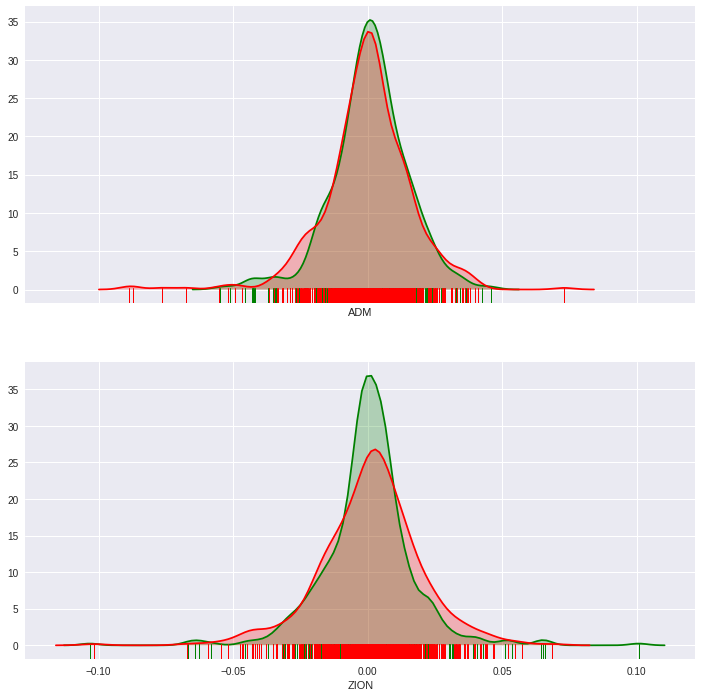
\includegraphics[scale=0.7]{img/anomalie_vs_normal_nss.png}
 \label{anormm}
\end{figure}

On peut bien noter les différences entre distribution normales et anormales soulignées par la méthode de détection par isolation. Cependant cette approche est à prendre avec prudence du faite de l'étape intermédiaire d'estimation non paramétrique des lois de probabilité des rendements.

%\subsection{Isolation des formes des courbes de distributions}

% system.time(sols <- lapply(df_den,solsf,de = de, OF=OF))
%utilisateur     système      écoulé 
%    6849.47        0.08     6851.69 

% part  (end)